%%%%%%%%%%%%%%%%%%%%%%%%%%%%%%%%%%%%%%%%%%%%%%%%%%%%%%%%%%%%%%%%%%%%%%%%%%%%%%%%%%%%%%%%%%%%%%%%%%%%%%%
% PACKAGES

\documentclass[a4paper, 11pt]{article}
\usepackage[utf8]{inputenc}
\usepackage[T1]{fontenc}
%\usepackage[catalan]{babel}
\usepackage{amsmath, amssymb, amsthm}
\usepackage[margin=1in]{geometry}
\usepackage{enumerate}
\usepackage{array}
\usepackage{graphicx}
\usepackage{ragged2e}
\usepackage{subfig}
\usepackage{caption}
\usepackage{subcaption}
\usepackage[dvipsnames]{xcolor}
\usepackage{float}
\usepackage{chngcntr}
\usepackage{ragged2e}
\usepackage{multirow}
\usepackage{vmargin}
\usepackage{hyperref}
\usepackage{url}
\usepackage{fancyhdr}
\usepackage{bigints}
\usepackage{listings}
\usepackage{xcolor,colortbl}

%%%%%%%%%%%%%%%%%%%%%%%%%%%%%%%%%%%%%%%%%%%%%%%%%%%%%%%%%%%%%%%%%%%%%%%%%%%%%%%%%%%%%%%%%%%%%%%%%%%%%%%
% COLORS

\definecolor{bluebell}{rgb}{0.64, 0.64, 0.82}
\definecolor{atomictangerine}{rgb}{1.0, 0.6, 0.4}
\definecolor{applegreen}{rgb}{0.55, 0.71, 0.0}
\definecolor{frenchblue}{rgb}{0.0, 0.45, 0.73}
\definecolor{darkpastelgreen}{rgb}{0.01, 0.75, 0.24}
\definecolor{darkpastelblue}{rgb}{0.47, 0.62, 0.8}
\definecolor{navy}{rgb}{0,0,128}
\definecolor{codegreen}{rgb}{0,0.6,0}
\definecolor{codegray}{rgb}{0.5,0.5,0.5}
\definecolor{codepurple}{rgb}{0.58,0,0.82}
\definecolor{backcolour}{rgb}{0.95,0.95,0.92}
\definecolor{amaranth}{rgb}{0.9, 0.17, 0.31}
\definecolor{GRAY}{rgb}{0.75, 0.75, 0.75}
\definecolor{deepfuchsia}{rgb}{0.76, 0.33, 0.76}
\definecolor{deepmagenta}{rgb}{0.8, 0.0, 0.8}
\definecolor{funcblue}{rgb}{0.36, 0.57, 0.9}

%%%%%%%%%%%%%%%%%%%%%%%%%%%%%%%%%%%%%%%%%%%%%%%%%%%%%%%%%%%%%%%%%%%%%%%%%%%%%%%%%%%%%%%%%%%%%%%%%%%%%%%
% SETTINGS

% COLOR LINK/REFERENCES
\hypersetup{colorlinks=true,
            linkcolor=blue,
            filecolor=magenta,      
            urlcolor=blue,
            }

% PAGE'S STYLE OF INITIAL PAGES
\fancypagestyle{plain}{
    \lhead[]{} % left part of the header
    \rhead[]{} % right part of the header
    \fancyfoot[]{} % borrow the foot counter page
    \lfoot[]{} % left part of the footpage
    \rfoot[]{} % right part of the footpage
    \renewcommand{\headrulewidth}{0pt} % separator line of the header
    \renewcommand{\footrulewidth}{0.5pt} % separator line of the footpage
}

% PAGE'S STYLE FOR THE THESIS
\fancypagestyle{extended_plain}{
    \lhead[]{Gerard Lahuerta Martín} % left part of the header
    \rhead[]{\leftmark} % right part of the header
    \fancyfoot[]{} % borrow the foot counter page
    \lfoot[]{} % left part of the footpage
    \rfoot[]{\thepage} % right part of the footpage
    \renewcommand{\headrulewidth}{0.5pt} % separator line of the header
    \renewcommand{\footrulewidth}{0.5pt} % separator line of the footpage
}

%%%%%%%%%%%%%%%%%%%%%%%%%%%%%%%%%%%%%%%%%%%%%%%%%%%%%%%%%%%%%%%%%%%%%%%%%%%%%%%%%%%%%%%%%%%%%%%%%%%%%%%
% CODE STYLE


%%%%%%%%%%%%%%%%%%%%%%%%%%%%%%%%%%%%%%%%%%%%%%%%%%%%%%%%%%%%%%%%%%%%%%%%%%%%%%%%%%%%%%%%%%%%%%%%%%%%%%%
% DOCUMENT

\begin{document}
\pagestyle{plain}

% TITLE
\begin{titlepage}
    \centering
    {
\includegraphics[width=0.4\textwidth]{PORTADA/UAB.png}\par}
    \vspace{1cm}
    {\bfseries\LARGE \href{https://www.uab.cat/}{Universitat Autònoma de Barcelona} \par}
    \vspace{2cm}
    {\Large Degree Thesis \par}
    \vspace{2em}
    \rule{\linewidth}{0.4pt}\\
    \vspace{1cm}
    {\scshape\Huge \textbf{Improvements of Deterministic Processes through Neural Networks} \par}
    \vspace{1cm}
    \rule{\linewidth}{0.4pt}\\
    \vspace{2cm}
    {\Large
    \begin{figure}[h]
    \centering
        \begin{minipage}{5cm} \centering % Minipagina para la tabla. 8 cm de ancho
            \begin{tabular}{c}
                Author: \\
                \href{https://github.com/Gerard-Lahuerta}{Gerard Lahuerta Martín}
            \end{tabular}
        \end{minipage}
        \hspace{3em}
        \begin{minipage}{5cm} \centering % Minipagina para la tabla. 8 cm de ancho
            \begin{tabular}{c}
                Supervisor: \\
                \href{https://mat.uab.cat/~alseda/}{Dr. Lluís Alsedà Soler}
            \end{tabular}
        \end{minipage}
    \end{figure}\par}
    \vspace{2cm}
    {\scshape 
        \begin{minipage}{10cm} \centering % Minipagina para la tabla. 8 cm de ancho
            A thesis submitted in fulfilment of the requirements
            for the degree of Computational Mathematics and Data Analytics in the
        \end{minipage} 
    \par} 
    \vspace{2em}
    {\scshape\Large \href{https://www.uab.cat/ciencies}{science faculty} \par}
    \vfill
    {\Large June 2024 \par}
\end{titlepage}


\justifying
\newpage
\textcolor{white}{a}
\newpage 

% PRE SECTIONS
\section*{Declaration of Authorship}
\newpage
\section*{Abstract}
\newpage
\section*{Acknowledgements}
I would like to express my gratitude to my family for their support throughout my thesis, degree, and my entire life.\\
\textcolor{white}{a}\\
I am especially grateful to my mother, Maria Montserrat, for her encouragement and guidance in facing the challenges of this thesis and my career.\\
\textcolor{white}{a}\\
Thanks to all the peoples that treatme as I was part of their family.\\
\textcolor{white}{a}\\
I also appreciate the encouragement and support of my colleagues.\\
\textcolor{white}{a}\\
Finally, I want to give a special mention to Dr. Lluís Alsedà for guiding me through the thesis and being an inspiration.\\
\textcolor{white}{a}\\
Thank you all for everything. 
\newpage

% CONTENTS
\tableofcontents
\listoffigures
\listoftables


\newpage \pagestyle{extended_plain}
\setcounter{page}{2}
\addcontentsline{toc}{section}{Introducción}
\section*{Introducción}
\newpage

\newpage
\section{Neural Networks} 
A neural Network is made of individual and independent elements connected between them, passing and managing the information through the network formed.\\
In this thesis we will focus on one of the simplest networks, a multilayer perceptron, to test the different methods of optimization.





% MULTILAYER POERCEPTRON
\subsection{Multilayer Perceptron and Perceptron neuron}
One of the simple Neural Networks to analyse is the Multilayer Perceptron\footnote{To obtain more information about Multilayer Perceptron functionability check the following \href{https://en.wikipedia.org/wiki/Multilayer_perceptron}{link}}.\\
It was first proposed by Frank Rosenblat\footnote{Frank Rosenblat, psychologist and father of deep learning, check its \href{https://en.wikipedia.org/wiki/Frank_Rosenblat}{biografy}.} in 1958 (nevertheless its approach did not learn either produce accurate results).
\begin{figure}[h]
    \begin{minipage}{9cm}
       \begin{center}
           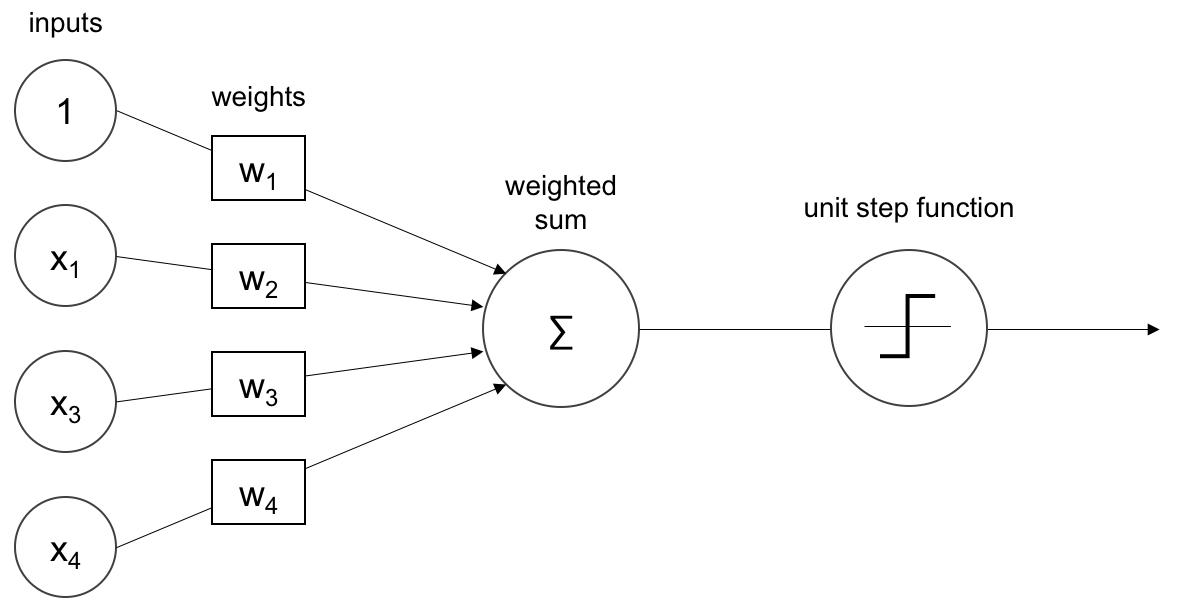
\includegraphics[width = 1 \textwidth]{Neural_Network/perceptron_schema.png}
           \caption{Schema of the Perceptron neuron}
       \end{center} 
    \end{minipage}
    \hspace{1em}
    \begin{minipage}{5cm}
        The Neural Network is made by individual neurons called \textit{Perceptrons}. The neurons are splitted into input, weight and activation functions.\\
        Nevertheless, the most important part of the neuron, and that determines significantly the capabilities of the neuron, is the activation function (which returns the output of the neuron).
    \end{minipage}
\end{figure}\\
The traditional activation function used in the Multilayer Perceptron is the Sigmoid: 
\begin{equation*}
    f(x) = \cfrac{1}{1+e^{-w\cdot x}},\text{ where: } x,w\in\mathbb{R}^n
\end{equation*}
The Multilayer Perceptron Topology can be splitted into layers of three types:
\begin{figure}[h]
    \begin{minipage}{9cm}
        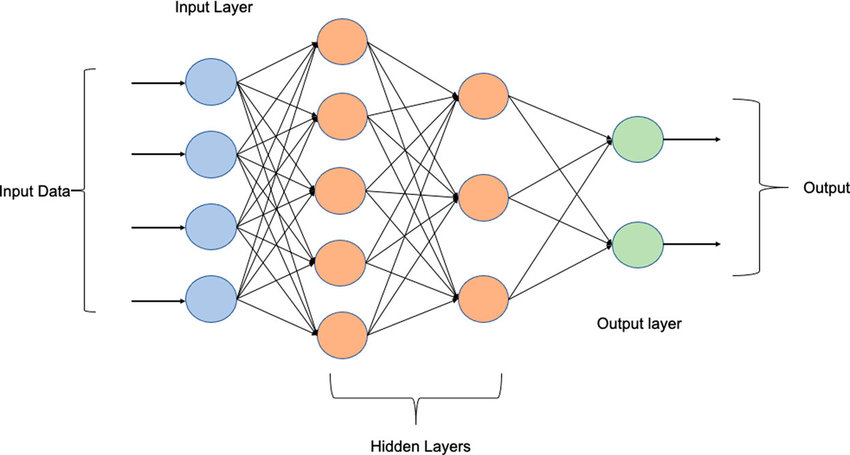
\includegraphics[width = 1 \textwidth]{Neural_Network/Multi-layer-perceptron-MLP-NN-basic-Architecture.png}
        \caption{Schema of the Multilayer perceptron}
    \end{minipage}
    \hspace{1em}
    \begin{minipage}{5cm}
        \begin{itemize}
            \item \textbf{Input Layer}: The initial set of neurons of the Multilayer Perceptron.
            \item \textbf{Output Layer}: The final set of neurons of the Multilayer Perceptron.
            \item \textbf{Hidden Layers}: The set of neurons (in layers) between the input and output layers.
        \end{itemize}
    \end{minipage}
\end{figure}\\
\newpage






% WHY WORKS
\subsection{Why Neural Networks works}
It is important to remark that what gives the capacity of model any system is because we can express everyproblem as a function (no matter if its a classification tasck, probability function, or prediction, regression function).\\
The association between a tasck and a function allow to apply the \textbf{Universal Approximation Theorem}.\\
\rule{\linewidth}{0.4pt}\\
\begin{itemize}
    \item \textbf{Definition:} Universal Approximation Theorem.
\end{itemize}  
For any function $f:\mathbb{R}^n \rightarrow \mathbb{R}^m$, with $m,n\in\mathbb{N}$, and a subset $D\subset \mathbb{R}^n$ where $f$ is continuous at all $D$, 
$\exists \{(w_i, b_i, c_i)\}_{i = 0}^k$ that: 
$$f(\vec{x}) - \lim_{k \rightarrow \infty} \sum_{i=0}^{k} c_i \sigma \left( w_i^T \cdot \vec{x} + b_i \right) = 0$$
Where $w_i \in \mathbb{R}^n$, $b_i\in \mathbb{R}$, $c_i \in \mathbb{R}^m$, $\vec{x}\in D$ and $\sigma$ the sigmoid function.\\
\rule{\linewidth}{0.4pt}\\\vspace{0.5em}
The parameters $\{w_i, b_i, c_i\}$ are associated (respectively) with the weights, bias and scale factor of the i-th neuron.\\
Neural Networks essentially use this theorem with a limit number of sigmoid (equal at de number of neurons), consecuently an error of approximation is given.
$$f(\vec{x})-\sum_{i=0}^{k} c_i \sigma \left( w_i^T \cdot \vec{x} + b_i \right) = \epsilon, k \in \mathbb{N}$$
Modeling systems the information of the function shape/tendency is limited or none, making only possible study the problem using data values.\\
This cases hare handle using the \textit{square-norm} metric (or \textit{Mean Squared Error}).\\
\rule{\linewidth}{0.4pt}
\begin{itemize}
    \item \textbf{Definition:} Square-norm: 
\end{itemize}
Being $f:\mathbb{R}^n \rightarrow \mathbb{R}^m$ function followed by the system.
Being $g:\mathbb{R}^n \rightarrow \mathbb{R}^m$, with $m,n\in\mathbb{N}$, as $g(\vec{x}) = \sum_{i=0}^{k} c_i \sigma \left( w_i^T \cdot \vec{x} + b_i \right)$.\\
Given a dataset $B = \{(\vec{x_i},\vec{y_i})\}_{i=0}^{N}$, with $N \in \mathbb{N}$, where $\forall (\vec{x_i},\vec{y_i}) \in B, \vec{y_i} = f(\vec{x_i})$.
$$\Delta^2 = \frac{1}{N} \sum_{i=0}^{N} \left( \vec{y_i} - g(\vec{x_i}) \right)^2$$
\rule{\linewidth}{0.4pt}\\\vspace{0.5em}
Decreassing the error $\Delta$ implies reducing the error $\epsilon$ because as $\Delta$ decrease the model improves its approximation whereas $\epsilon$ decrease.\\
As the more neurons are added into the Network, the approximation and the training time increases. This increase in training time for the model in cases is not worth it as it represents a minimum improvement of the model.\\
Moreover, the Backpropagation\footnote{The Backpropagation method is an algorithm to modify the internal parameters of a Neural network by using the chain rule, more information in the following \href{https://en.wikipedia.org/wiki/Backpropagation}{link}} method used to train Neural Networks have a complexity that increase the process time exponentially to the number of neurons.\\
Therefore, trying to obtain the ideal topology for solving a problem is a dificult tasck that in many cases resides about trial error.
\section{Neural Networks topology}
The main objective of the study is obtaining a more efficient process using neural networks than the traditional ways that has been used at time.\\
Doing this requires, as has been explained before, a non undertand process to obtain an eficient neural network.\\
Therefore, an observation has done while approaching this problem that could partial solve that non-undertand of what really is doing the neural network and deduce the optimal architecture. 
\subsection{Hypotesis and Proposal}
As has been said before, approaching this problem an intuitive idea apeared. \\
\rule{\linewidth}{0.4pt}
\begin{itemize}
    \item \textbf{Proposal:} If there is enough information about the system to model, exists an eficient neural network which architecture can be obtained using rules.
\end{itemize}
\rule{\linewidth}{0.4pt}\\ \vspace{0.5em}
The idea proposed is influenced by the following observations:
\begin{enumerate}
    \item Every deterministic process is a convination of restriccions that can be represented as a function.
    \item Every function can be splitted in domaind which its behavior can be categorized as: periodical, irrational, polinomical.
    \item The periodical, polinomical and irrational functions are continuous in "all"\footnote{In case of irrational functions such as $\sqrt{x}$, it can be interpretated as $f(x) = \left\{ \begin{matrix} 0, x < 0 \\ \sqrt(x), x \geq 0 \end{matrix} \right.$} domain.
    \item All continuous functions can be approximated using the \textbf{Universal Approximation Theorem}.
\end{enumerate}
Moreover, if a function does not follow one of this types of functions, it can be splited by more intervals until each of them can be aproximated by one of this types or even can be approximated using \textit{Fourier Series} or \textit{Taylor series} allowing it to be modeled by periodical and polinomical functions.\\
Therefore, this proposal can be verified reducing it into corroborate the following points:
\begin{enumerate}
    \item Each category of functions mencioned can be modeled using a particular architecture of neural network.
    \item Exists a determined minimum number of data registers were the neural network can be trained.  
\end{enumerate}
To verify the proposal a topological, efficiency and preccision studies is required.

\newpage
\subsection{Study of deterministic process}
To start, lets assume the following axioms to simplify the study and give some feedback to make the correlations to werify or dimsmiss the proposal.
\begin{enumerate}
    \item All periodically functions can be approximated as a convination of sinus functions.
    \item All polinomical functions can be approximated as a convination of lineal functions.
    \item All irrational functions can be approximated as a convination of irrational functions.
\end{enumerate}
All point can be proven using \textit{Taylor Series} and \textit{Fourier Series}.
Therefore, the study will be reduced into take patterns of the architectures used to approximate the functions $\sin(x), \sqrt(x), x^2$.\\
This paper use $I-H-N-O$ nomenclature to represent the architecture of the neural network, where the letters $I,H,N,O$ represents the number of inputs, the hidden layers, the number of neurons for each hidden layer and the number of outputs respectively.

\subsubsection{Study of the \textit{sin} function}
To test if exists an architecture that can approximated efficiently the $\sin$ function in the real plane, will be study to approximated the function in the interval $[0, 2\pi]$ using a fixed number of iterations with diferents architectures.    
\begin{figure}[h]
    \centering
    \subfloat[Model 1-1-1-1]{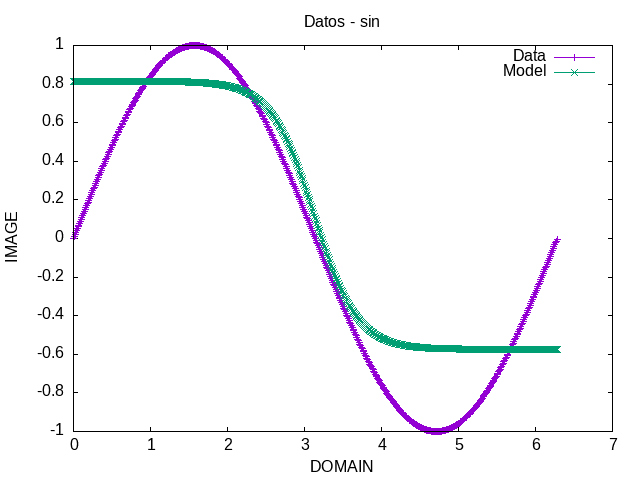
\includegraphics[width=0.24\linewidth]{img/sin/sin-1-1-1-1.png}}
    \subfloat[MSE 1-1-1-1]{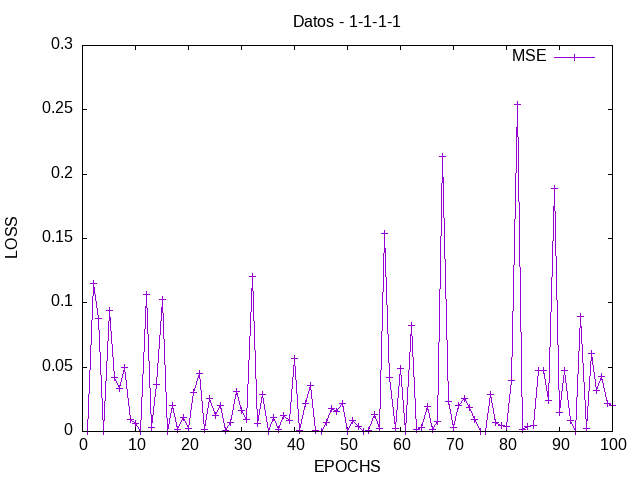
\includegraphics[width=0.24\linewidth]{img/sin/sin-loss-1-1-1-1.png}}
    \hspace{1em}
    \subfloat[Model 1-1-2-1]{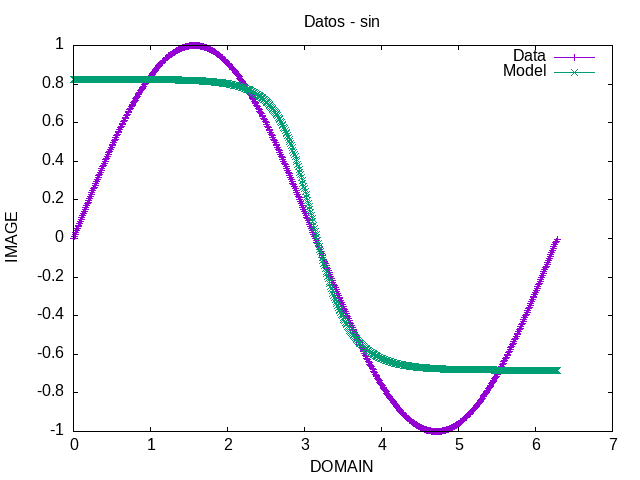
\includegraphics[width=0.24\linewidth]{img/sin/sin-1-1-2-1.png}}
    \subfloat[MSE 1-1-2-1]{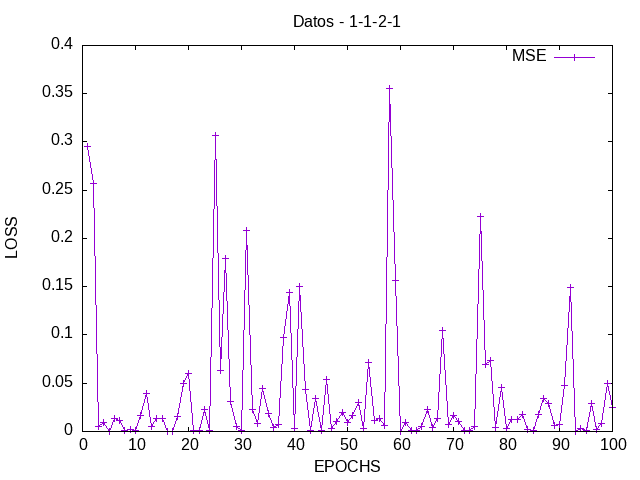
\includegraphics[width=0.24\linewidth]{img/sin/sin-loss-1-1-2-1.png}}
    \\
    \subfloat[Model 1-1-3-1]{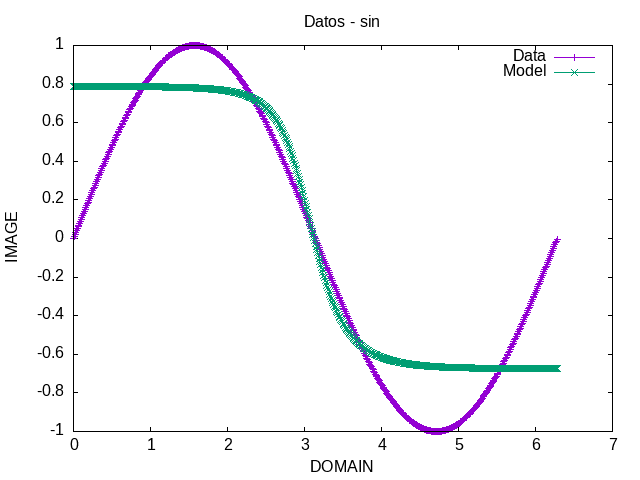
\includegraphics[width=0.24\linewidth]{img/sin/sin-1-1-3-1.png}} 
    \subfloat[MSE 1-1-3-1]{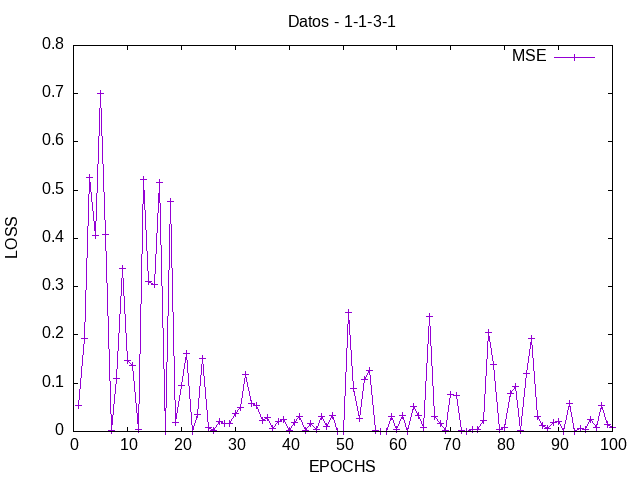
\includegraphics[width=0.24\linewidth]{img/sin/sin-loss-1-1-3-1.png}}
    \hspace{1em}
    \subfloat[Model 1-2-2-1]{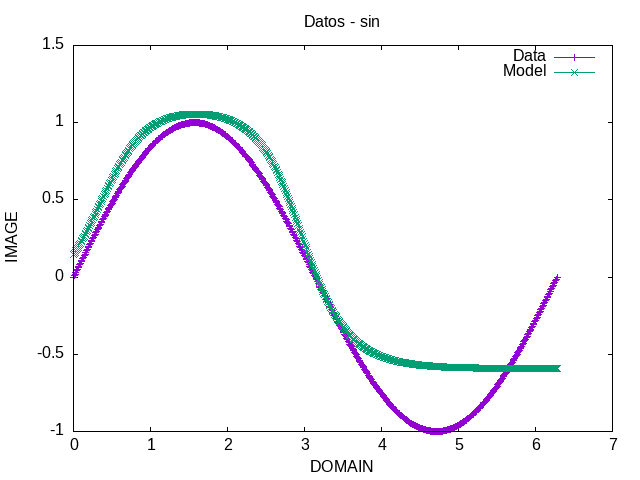
\includegraphics[width=0.24\linewidth]{img/sin/sin-1-2-2-1.png}}
    \subfloat[MSE 1-2-2-1]{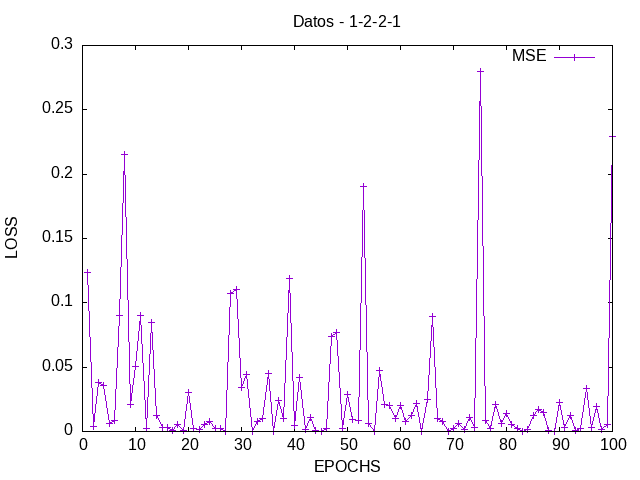
\includegraphics[width=0.24\linewidth]{img/sin/sin-loss-1-2-2-1.png}}
    \\
    \subfloat[Model 1-2-4-1]{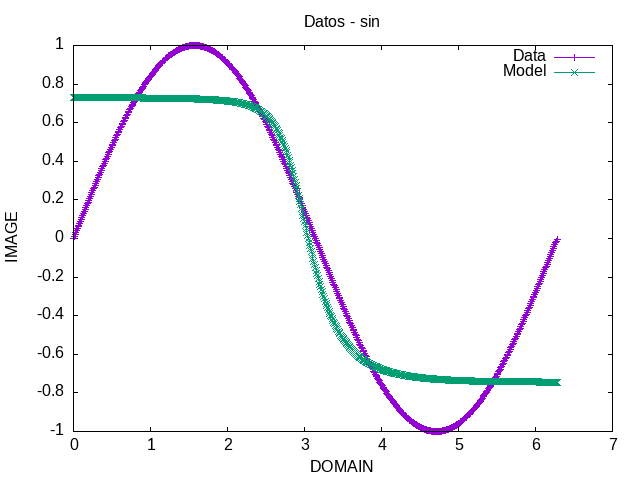
\includegraphics[width=0.24\linewidth]{img/sin/sin-1-2-4-1.png}}
    \subfloat[MSE 1-2-4-1]{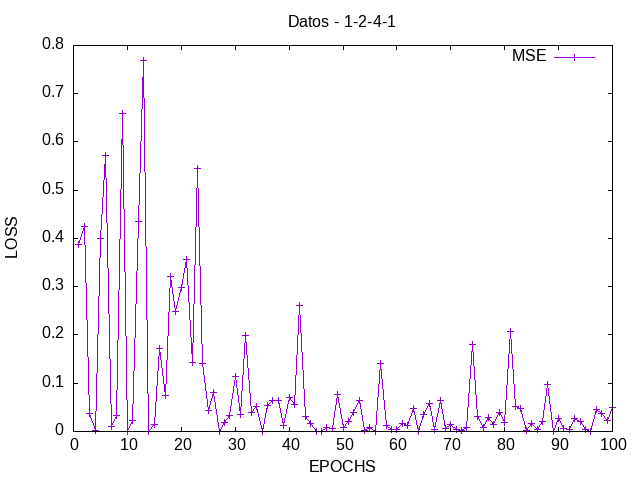
\includegraphics[width=0.24\linewidth]{img/sin/sin-loss-1-2-4-1.png}}
    \hspace{1em}
    \subfloat[Model 1-4-2-1]{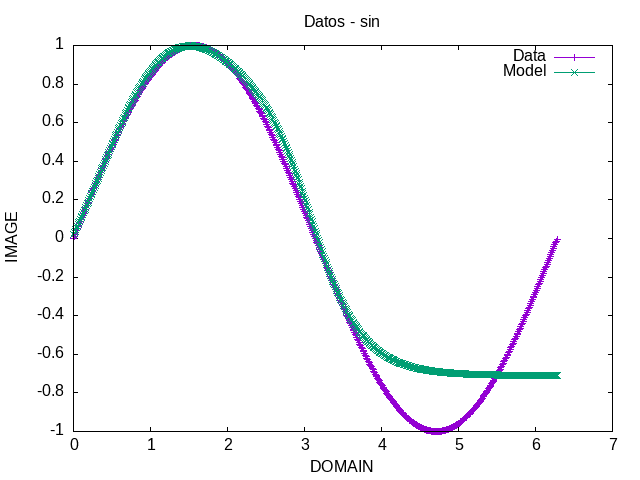
\includegraphics[width=0.24\linewidth]{img/sin/sin-1-4-2-1.png}}
    \subfloat[MSE 1-4-2-1]{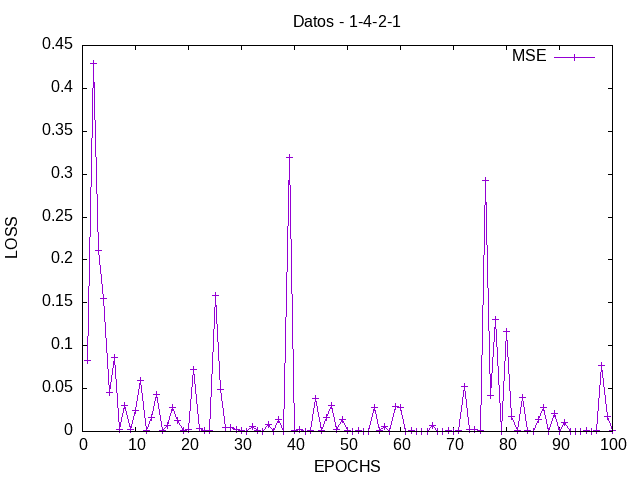
\includegraphics[width=0.24\linewidth]{img/sin/sin-loss-1-4-2-1.png}}
    \caption{Results of diferents architectures approximating the function \textit{sin}}
    \label{fsin100}
\end{figure}\\
The results shown in Figure \ref{fsin100} where obtained fixing 100 epochs and trained using the stochastic gradient descend method with a learning rate of $0.1$ trying to minimice the \textit{Square-norm} error (\textit{MSE}).\\
As can be seen in the Figure, almost all architectures does not approximate the $\sin$ function properly, despite the architectures \textit{1-2-2-1} and \textit{1-4-2-1}.\\
If the experiment is repeated changing the epoch number (insted of 100 change to 200) the results are almost similar (with more precission in some parts but no improvement of modelation).\\
However, the architectures \textit{1-4-4-1} and \textit{1-4-2-1} give an augment of precission significally important.
\begin{figure}[h]
    \subfloat[Model 1-2-4-1]{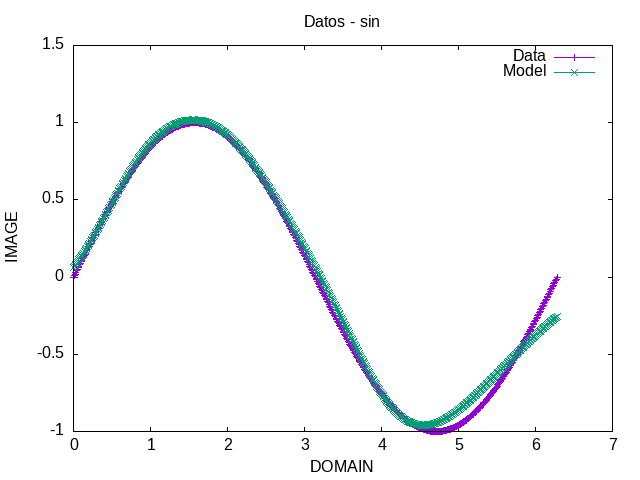
\includegraphics[width=0.24\linewidth]{img/sin/sin-1-4-2-1(200).png}}
    \subfloat[MSE 1-2-4-1]{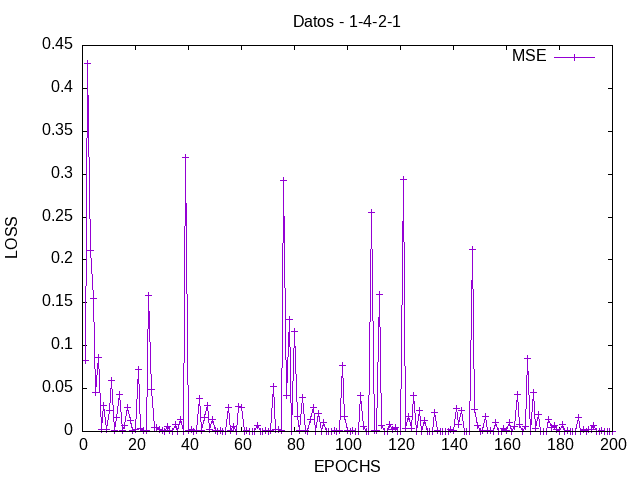
\includegraphics[width=0.24\linewidth]{img/sin/sin-loss-1-4-2-1(200).png}}
    \hspace{1em}
    \subfloat[Model 1-4-4-1]{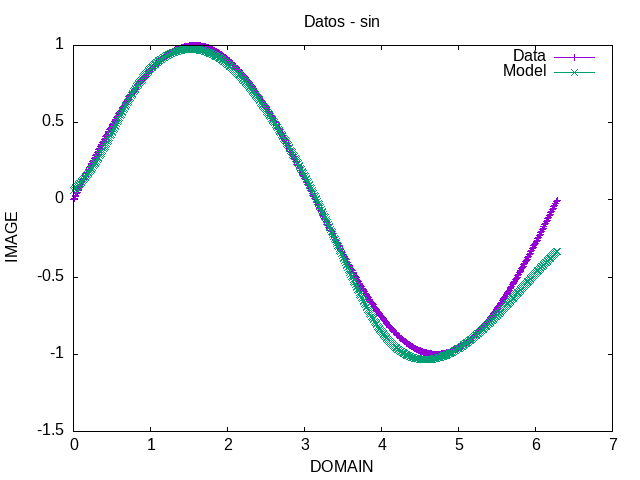
\includegraphics[width=0.24\linewidth]{img/sin/sin-1-4-4-1(200).png}}
    \subfloat[MSE 1-4-4-1]{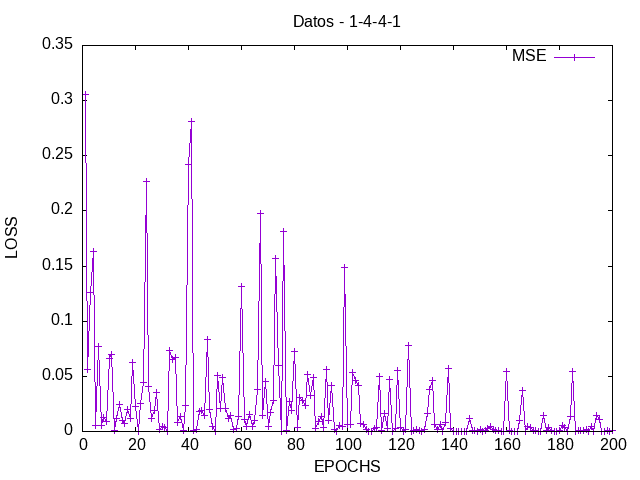
\includegraphics[width=0.24\linewidth]{img/sin/sin-loss-1-4-4-1(200).png}}
    \caption{Architectures that improves the modelation of \textit{sin} function}
    \label{fsin200}
\end{figure}\\
The approximation done by these architectures is so significant that allow to observe and conclut that the model that approximates the best the $\sin$ function if 1-2-4-1.\\
This conlusion is obtained because is the minimum architecture that can approximate the function, that can "learn"\footnote{Learn in this tearm refears as if the training process allow to reduce the loss (also named error) near 0 with a significally decrease throughout the epochs.}.\\
Moreover, it can be an evidence of the following proposal:\\
\rule{\linewidth}{0.4pt}
\begin{itemize}
    \item \textbf{Proposal:} To approximate any periodical function in real plane needs minimum 2 neurons in each of the $2\cdot K$ hiddden layers, where $K$ is sum of relatives extrems and point of inflection of the function.
\end{itemize}
\rule{\linewidth}{0.4pt}\\ \vspace{0.5em}
This proposal is obtained observing that every layer of the neural netwrok is modeling one interval (delimited by the extreams of the function and inflection points) and for perform that approximation nead at least 2 sigmoids.
\subsubsection{Study of the \textit{parabolic} function}
The same experiment have been done with the function $x^2$ (and also the $x^3$ to have more results to compare) with fixed epochs, learning rate and domain.\\
Concretly, the values of epochs, learning rate and domain used are, respectively, $100$, $0.1$ and $[-2,2]$.\\
The results obtained for polinocmical functions are shown in \ref{poli100}.
\begin{figure}[h!]
    \centering
    \subfloat[\centering Model\\1-1-1-1]{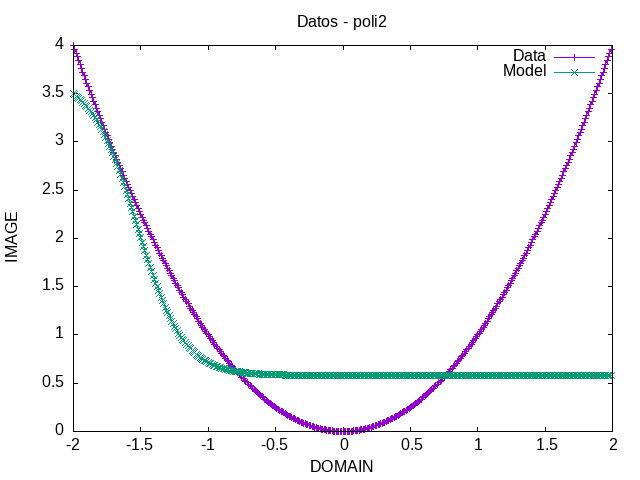
\includegraphics[width=0.15\linewidth]{img/poli/poli2-1-1-1-1.png}}
    \subfloat[\centering MSE\\1-1-1-1]{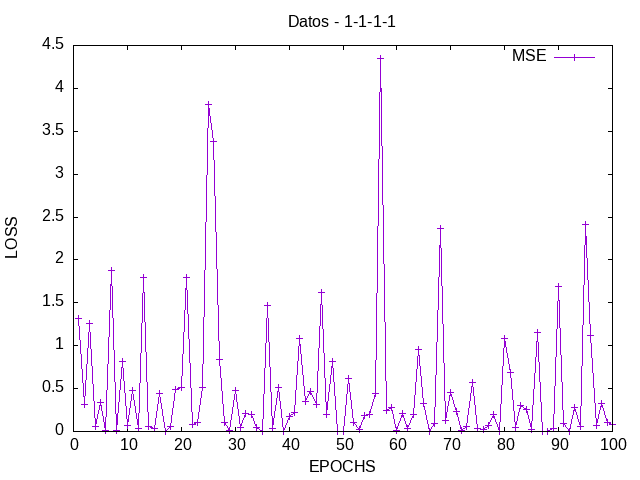
\includegraphics[width=0.15\linewidth]{img/poli/poli2-loss-1-1-1-1.png}} \hspace{0.5em}
    \subfloat[\centering Model\\1-2-1-1]{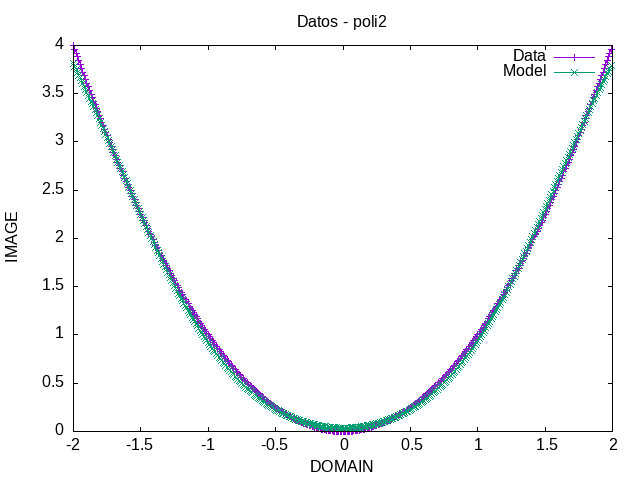
\includegraphics[width=0.15\linewidth]{img/poli/poli2-1-2-1-1.png}}
    \subfloat[\centering MSE\\1-2-1-1]{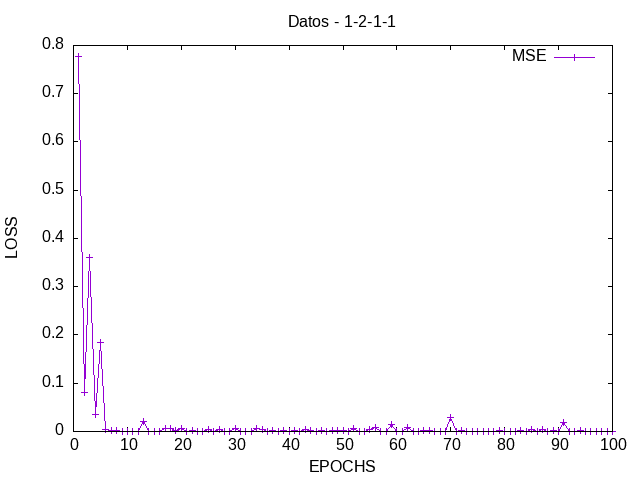
\includegraphics[width=0.15\linewidth]{img/poli/poli2-loss-1-2-1-1.png}} \hspace{0.5em}
    \subfloat[\centering Model\\1-2-2-1]{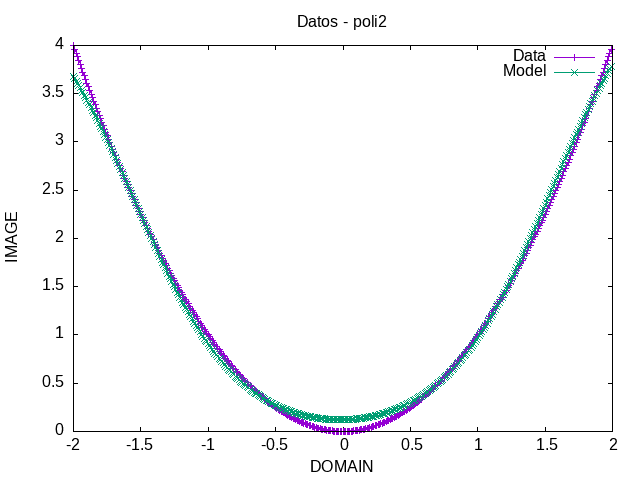
\includegraphics[width=0.15\linewidth]{img/poli/poli2-1-2-2-1.png}}
    \subfloat[\centering MSE\\1-2-2-1]{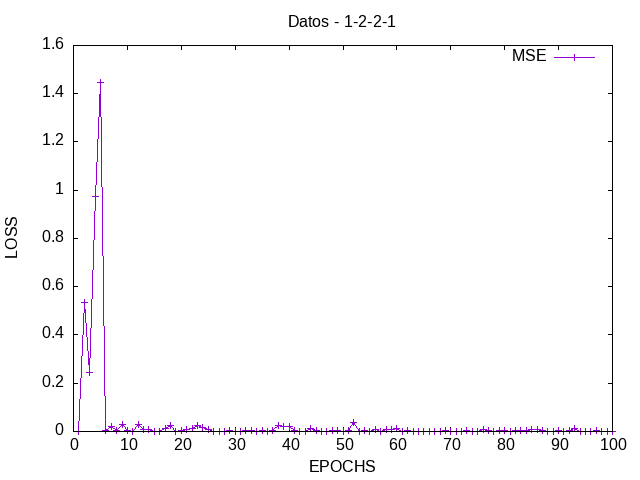
\includegraphics[width=0.15\linewidth]{img/poli/poli2-loss-1-2-2-1.png}}
    \\\vspace{1em}
    \subfloat[\centering Model\\1-1-1-1]{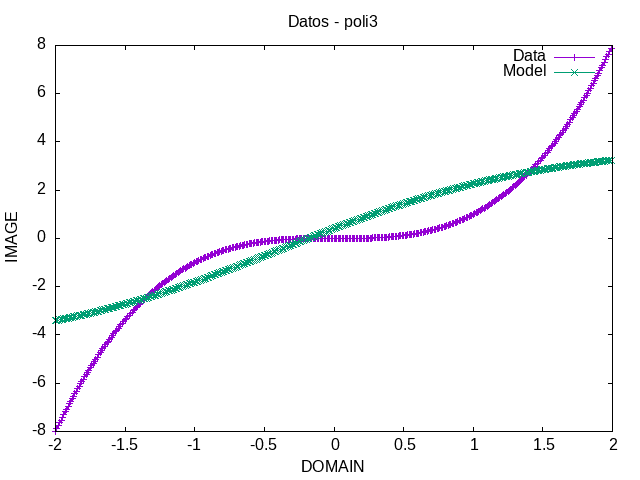
\includegraphics[width=0.15\linewidth]{img/poli/poli3-1-1-1-1.png}}
    \subfloat[\centering MSE\\1-1-1-1]{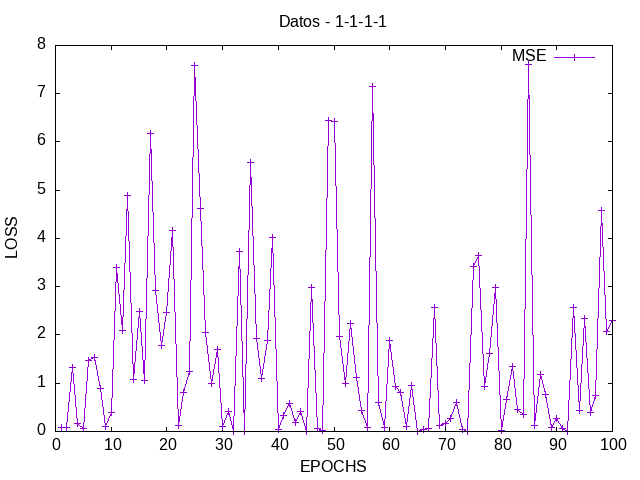
\includegraphics[width=0.15\linewidth]{img/poli/poli3-loss-1-1-1-1.png}} \hspace{0.5em}
    \subfloat[\centering Model\\1-2-1-1]{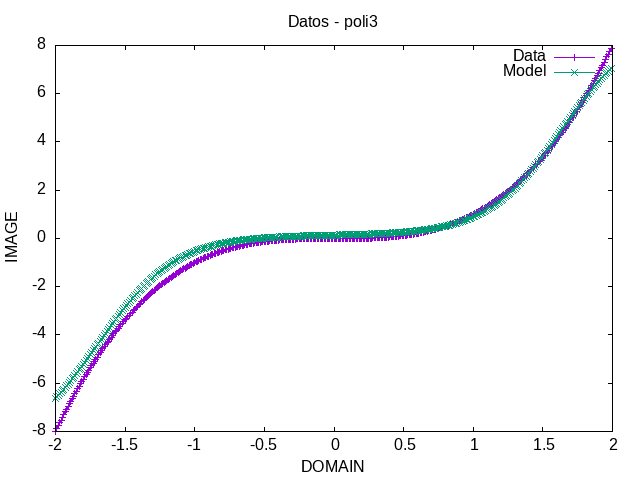
\includegraphics[width=0.15\linewidth]{img/poli/poli3-1-2-1-1.png}}
    \subfloat[\centering MSE\\1-2-1-1]{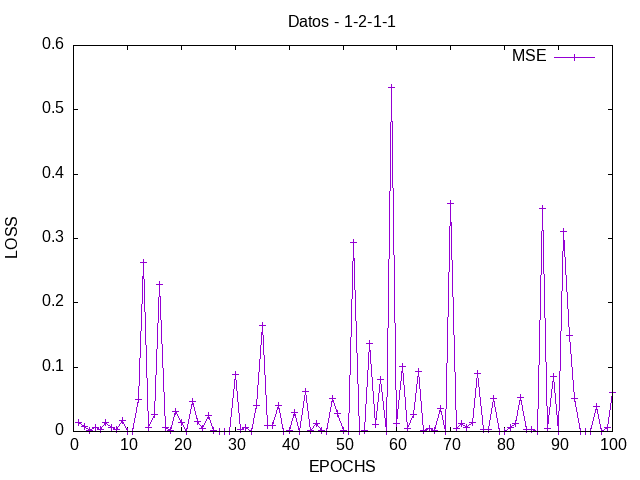
\includegraphics[width=0.15\linewidth]{img/poli/poli3-loss-1-2-1-1.png}} \hspace{0.5em}
    \subfloat[\centering Model\\1-2-2-1]{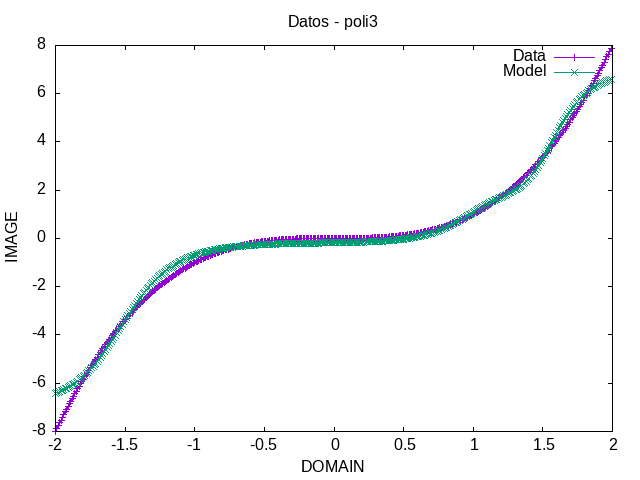
\includegraphics[width=0.15\linewidth]{img/poli/poli3-1-2-2-1.png}}
    \subfloat[\centering MSE\\1-2-2-1]{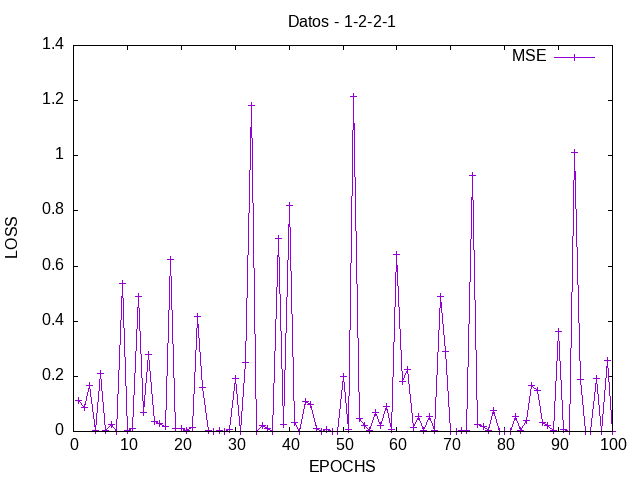
\includegraphics[width=0.15\linewidth]{img/poli/poli3-loss-1-2-2-1.png}}
    \caption{Results of diferents architectures approximating the functions $x^2$ and $x^3$}
    \label{poli100}
\end{figure}\\
It shows how the most efficient architecture (which give the better performance as modeling as precission) is the $1-2-1-1$.\\
This architecture is similar obtained before with the periodical functions but is not the same, which was one of the axioms suposed in the proposal.\\
Therefore, a last study will be done to obtain the architecture need to model the irrational functions.
\newpage
\subsubsection{Study of the \textit{squared root} function}
Finally, reproducing the experiment for the function $\sqrt{x}$, the results obtained are shown in \ref{sqrt100}.
\begin{figure}[h]
    \centering
    \subfloat[Model 1-1-1-1]{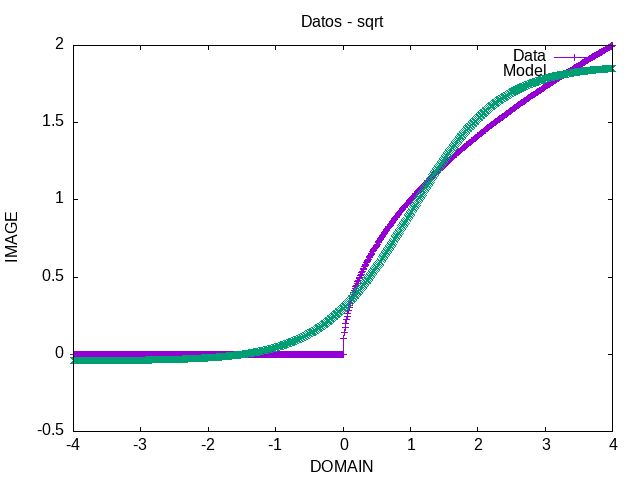
\includegraphics[width=0.24\linewidth]{img/sqrt/sqrt-1-1-1-1.png}}
    \subfloat[MSE 1-1-1-1]{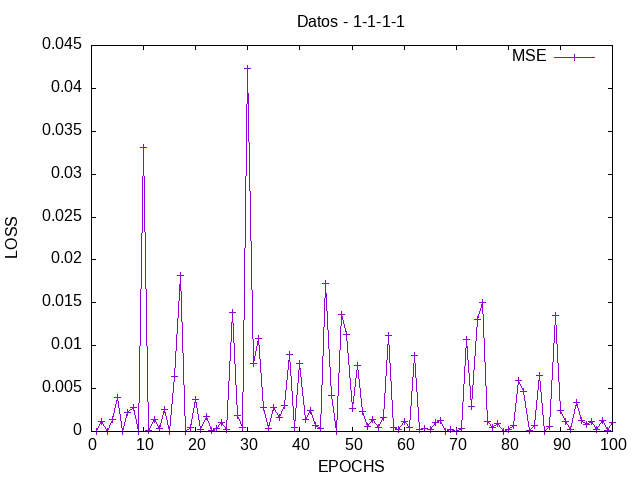
\includegraphics[width=0.24\linewidth]{img/sqrt/sqrt-loss-1-1-1-1.png}}
    \hspace{1em}
    \subfloat[Model 1-1-2-1]{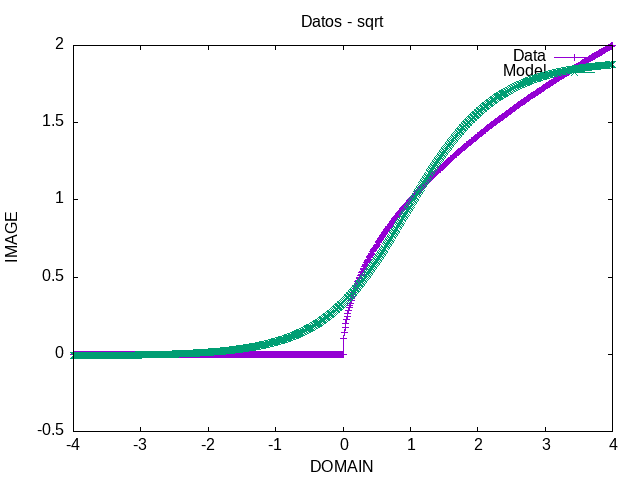
\includegraphics[width=0.24\linewidth]{img/sqrt/sqrt-1-1-2-1.png}}
    \subfloat[MSE 1-1-2-1]{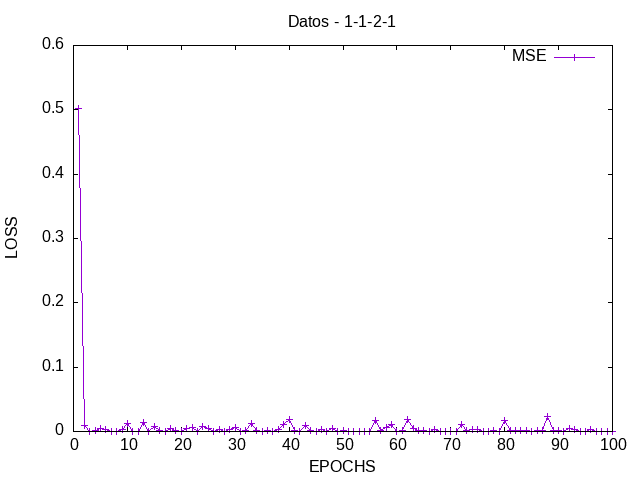
\includegraphics[width=0.24\linewidth]{img/sqrt/sqrt-loss-1-1-2-1.png}}
    \\
    \subfloat[Model 1-2-1-1]{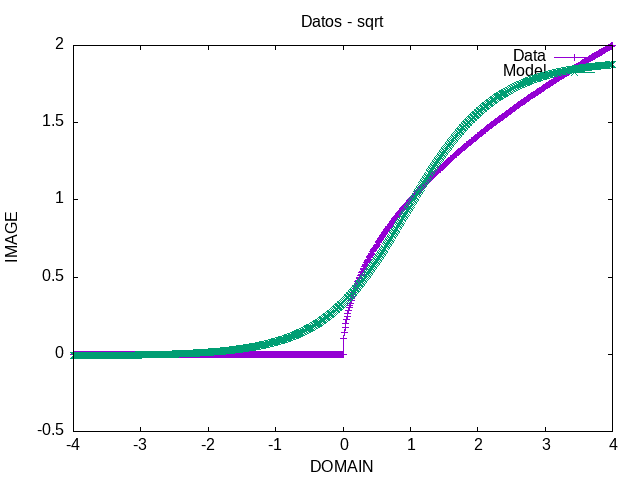
\includegraphics[width=0.24\linewidth]{img/sqrt/sqrt-1-2-1-1.png}} 
    \subfloat[MSE 1-2-1-1]{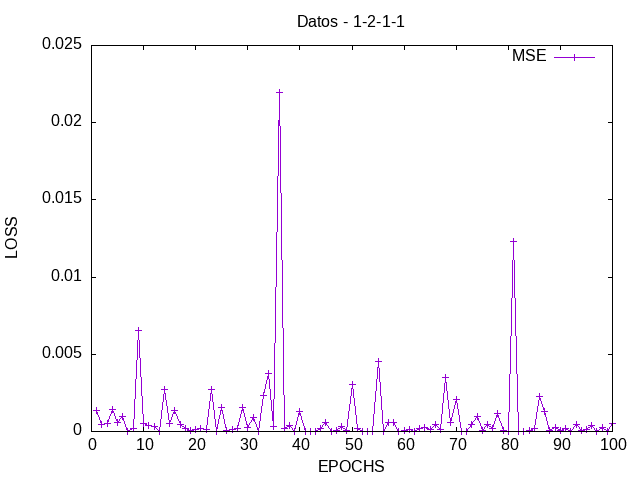
\includegraphics[width=0.24\linewidth]{img/sqrt/sqrt-loss-1-2-1-1.png}}
    \hspace{1em}
    \subfloat[Model 1-3-1-1]{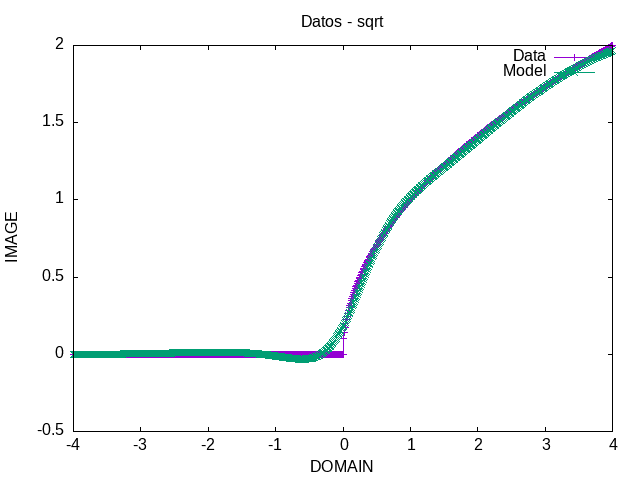
\includegraphics[width=0.24\linewidth]{img/sqrt/sqrt-1-3-1-1.png}}
    \subfloat[MSE 1-3-1-1]{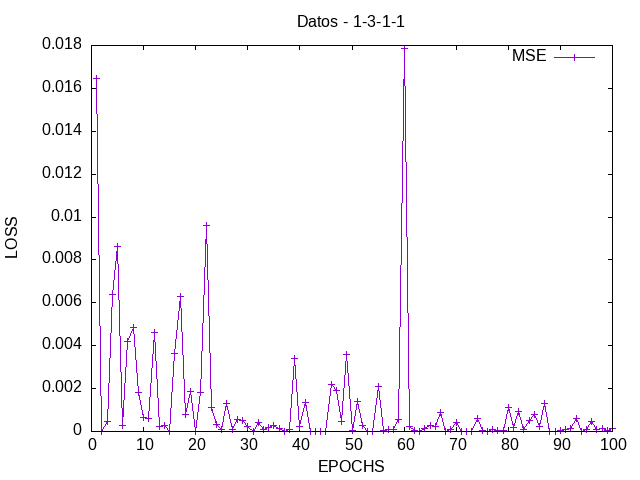
\includegraphics[width=0.24\linewidth]{img/sqrt/sqrt-loss-1-3-1-1.png}}
    \caption{Results of diferents architectures approximating the function $\sqrt{x}$}
    \label{sqrt100}
\end{figure}\\
In this study, the only parameters that where changed respect the previous experiments was the domain (which was increased to the interval $[-4,4]$).\\
As it can be observed, the architecture that approximate the best the function is $1-3-1-1$.\\
Moreover, comment that the intutition of the inclusion of irrational funccions such as the $\sqrt{x}$ in the axioms of the proposal was made to use the property of having a function similar to $ReLU$\footnote{The \textit{ReLU} function is widely use as an activation function which is deffined as $f(x) = \left\{ \begin{matrix} 0, x < 0 \\ x, x\geq 0\end{matrix} \right.$}.\\
This inclusion of the function $\sqrt(x)$ in spite of the $ReLU$ was made thinking that was a better option and the least "forced" option of any other function that could give that similar property. However, this text between other similar functions was not made so could be interesting to expand this stuidy adding and experiment with other functions.
\subsection{Viability of approximation discontinuous functions}
It is important to have in mind that splitting functions in domains can develop in discontinuities which does not allow the use of the \textbf{Universal Approximation Theorem}.\\
Nevertheless the application of neural networks in tascks such as classification or regression in many areas, with no information of the function that are approximating, using activation functions diferent from the \textit{sigmoid} that give (apparently) correct results give the idea that possibly the theorem could be expanded and (in some cases) have no need of the continuity restriction.\\
\rule{\linewidth}{0.4pt}
\begin{itemize}
    \item \textbf{Proposal:} If a function has discontinuities diferent from asimptotyc, the \textbf{Universal Approximation Theorem} can be used to give an approximation with error 0 when the number of sigmoid tends to infinity.
\end{itemize}
\rule{\linewidth}{0.4pt}\\ \vspace{0.5em}
This proposal can be sustain by the ability of sigmoid functions to approximate jump discontinuities. However, an experiment with discontinuous functions have done to give evidence of this proposal.
\subsubsection{Study of Jump discontinuity}
In this experiment a simple architecture of $1-2-2-1$ with high amount of epochs (concretly $10000$) and fixed learning rate of $0.1$ have been used to approximated the function:
$$ f(x) = \left\{ \begin{matrix}
    1, x \leq 1 \\
    0, x \in (1,2] \\
    -1, x > 2
\end{matrix} \right. $$
The results of approximating the function in the interval $[0,3]$ are shown in \ref{disc}.
\begin{figure}[h]
    \centering
    \subfloat[Model]{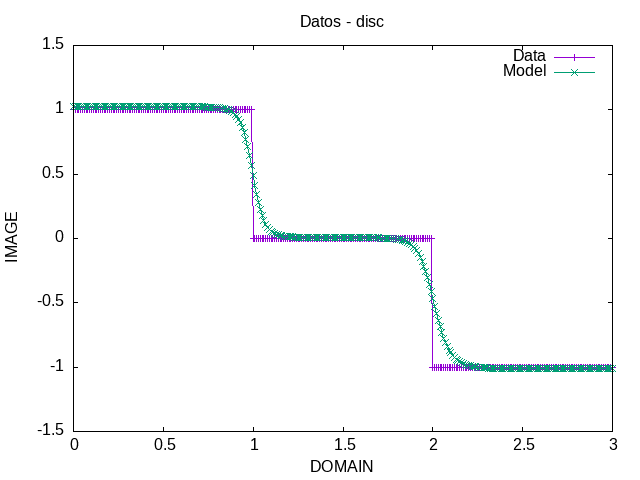
\includegraphics[width=0.5\linewidth]{img/disc/disc-1-2-2-1.png}}
    \subfloat[MSE]{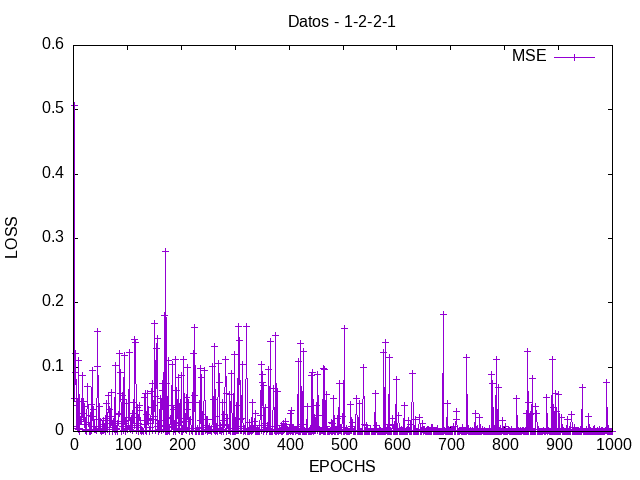
\includegraphics[width=0.5\linewidth]{img/disc/disc-loss-1-2-2-1.png}}
    \caption{Architecture $1-2-2-1$ approximation to a jump discontinuity function}
    \label{disc}
\end{figure}\\
As can be seen in the figure \ref{disc}, using a limited model with enough number of epochs the approximation is quiet acceptable. Therefore the use of \textit{sigmoid} functions in approximate splitted functions with jump discontinuities can be use at least in some cases.
\subsubsection{Study of Asimptotyc discontinuity}
However, the application of the \textbf{Universal Approximation Theorem} in discontinuities such as asimptotyc can give problems that impossibilates the modelation using sigmoids.\\
Repeating the experiment done with the jump discontinuity function, but with a more prowerfull architecture, to approximate the function $\tan{x}$ in the interval $[-\frac{\pi}{2},\frac{\pi}{2}]$ give us an idea of this problem.\\
The results obtained are shown in \ref{asymp}.
\begin{figure}[h]
    \centering
    \subfloat[Model]{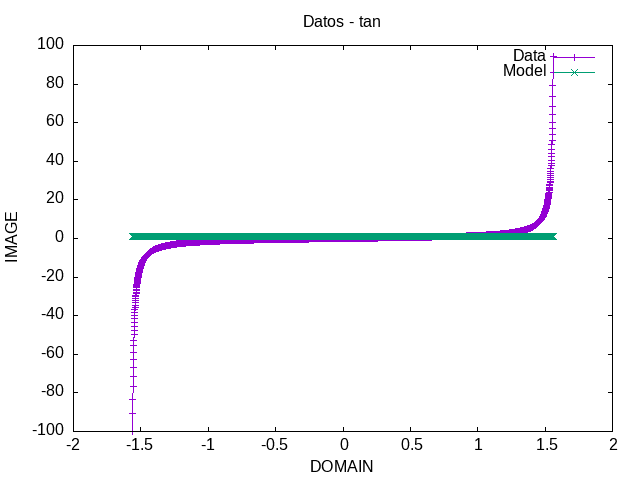
\includegraphics[width=0.5\linewidth]{img/disc/tan-1-5-5-1.png}}
    \subfloat[MSE]{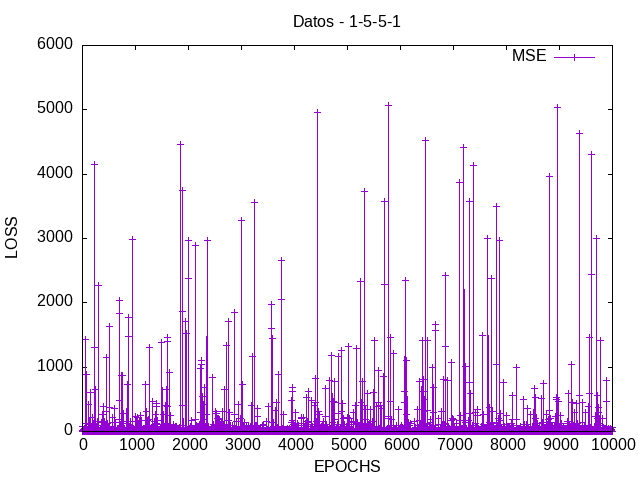
\includegraphics[width=0.5\linewidth]{img/disc/tan-loss-1-5-5-1.png}}
    \caption{Architecture $1-5-5-1$ approximation to $\tan{x}$ function}
    \label{asymp}
\end{figure}\\
As can be observed the neural network is limited and cannot approximate properly the function. However, the use of other activation function such as the $ReLU$ mentioned before can give a better performance.\\
In case of using the $ReLU$ function, it give another problem that can be dificult to handle, the \textbf{Universal Approximation Theorem} does not ensure that the resulting function approximates with a limited error the system.\\
Moreover, the use of the \textit{BackPropagation} method and its dependency with the \textit{Newtons Method} (the \textit{Steepest Gradient Descend}) to obtain zeros of the \textit{cost function} in the training process, does not ensure that the solution it arrive is the best or, even doe, if it is correct in all cases (and we can be blind in situations were the network was not tested).
\subsection{Observations of the results}
To sump up all the results and conlusions obtained in the studies we can conclud if theres enough evidence of the proposal.\\
\rule{\linewidth}{0.4pt}
\begin{itemize}
    \item \textbf{Proposal:} If there is enough information about the system to model, exists an eficient neural network which architecture can be obtained using rules.
\end{itemize}
\rule{\linewidth}{0.4pt}\\ \vspace{0.5em}
To verify the viability of the proposal needed to acomplish the following conditions:
\newpage
\begin{enumerate}
    \item \underline{All periodically functions can be approximated as a convination of sinus functions.}\\
    The first contidion can be proven usen \textit{Fourier series}\\
    However, its important to mention that a periodical function such as $\tan{x}$ can not be approximated due to the asymptoties. 
    Therefore could exist a periodical function that can be modeled with $\sin$ functions because it requeres that can hadle asymptoties.\\
    \item \underline{All polinomical functions can be approximated as a convination of lineal functions.}\\
    Such as the first condition, the second one can be proven using \textit{Taylor Series}, not having a possible counter part that do not apply.\\
    \item \underline{All irrational functions can be approximated as a convination of irrational functions.}\\
    The point 3 can be explained using the condition that we are tryiung to approximate a function un a certain interval. Therefore iy can be obtained the following deduction:\\
    \rule{\linewidth}{0.4pt}
    \begin{itemize}
        \item \textbf{Deduction:} Approximation of irration functions.\\
        Being $f_n:\mathbb{R}\rightarrow\mathbb{R}$, $g:\mathbb{R}\rightarrow\mathbb{R}$ where $f_n(x) = \sqrt[n]{x}, \forall n \in \mathbb{N} / n > 1$ and $g(x) = \sqrt{x}$.\\
        $$ \exists c,d \in \mathbb{R} / \forall x \in [a,b], f_n(x)- g(c\cdot x + d) < \epsilon$$ 
        Where $\epsilon\in\mathbb{R^+}$ is the error and $\{ c,d \}$ are parameters that ajust $g$ to approximate $f_n$ in the interval $[a,b]\cup \mathbb{R}$.
    \end{itemize}
    \rule{\linewidth}{0.4pt}\\
    Nevertheless, mention that when $n$ (the degree of the root) is even the interval needs to be in the set $\mathbb{R^+}$. Moreover, this deduction can handle situations when the set of functions $f_n$ are defined as $f(x)_n = \alpha \sqrt[n]{x} + \beta$ where the parameters $\alpha,\beta \in \mathbb{R}$ \\
    This deduction can also be demostrated using tangency:\\
    \rule{\linewidth}{0.4pt}
    \begin{itemize}
        \item \textbf{Demostration:} Approximation of irration functions.\\
        Being $f_n:\mathbb{R}\rightarrow\mathbb{R}$, $g:\mathbb{R}\rightarrow\mathbb{R}$ where $f_n(x) = \sqrt[n]{x}, \forall n \in \mathbb{N} / n > 1$ and $g(x) = \sqrt{x}$.\\
        Being $P=(p_0, p_1) / p_0 = \frac{a+b}{2}, p_1 = f_n(p_0)$, $\exists c,d\in\mathbb{R} / g(c\cdot p_0 + d) = p_1$.
        Therefore, 
        $$\exists (\alpha, \beta) \subset [a,b] / p_0 = \frac{\alpha + \beta}{2} \text{ where } \forall x \in (\alpha, \beta), f_n(x) - g(c\cdot x + d) < \epsilon$$
        $\epsilon\in\mathbb{R^+}$ the error.
    \end{itemize}
    \rule{\linewidth}{0.4pt}\\
    These demostration could be use for every function, not limiting them only for irrational functions.
\end{enumerate}
\begin{enumerate}
    \setcounter{enumi}{3}
    \item \underline{The mencioned functions can be modeled using a particular architecture.}\\
    The studies about the differents architectures of the diferents functions ($x^2, \sin{x}, \sqrt{x}$) shows that exist a diferenciable minimum architecture that approximate the best each function.\\
    \item \underline{Exists a determined minimum number of data to train the neural network.}\\
    That point is controversial. In all the studies perfom the number of data available where diferents  with at least $200$ registers. However, the rellevant part about this is that it really needs a deterministic process that generates the dataset.\\
    Te minim information that is required is the determinmistic process intrinsecly. If there is no deterministic process the information needed will not be enough despite how many it could recap.\\
    This is consecuence of the backpropagation method and its dependency in the \textit{Steepest Gradient Descend}. If there is no "correct" model to compare and interpretate the functionability of the network it is not possible to "extract theoretically the best architecture".\\
    Hence, there is no "minim number of samples" despite there is a necessary existance of a (deterministic) \textit{non-black box}\footnote{A \textit{black box} model is a process where the internal operations and functionability of it can not be interpretated partially or at all, giving the aspect of being a non undertanable or/and verified model.} method.
\end{enumerate}
Concluding the observations, the studies give the enough evidence of the proposal.\\
To give more evidence of that proof, an experimental process will be done to extract th best minimal architecture that approximate a deterministic process.\\
Moreover, a efficiency test will be also perfomed to ensure that neural networks in colaboration with the information that gives the deterministic process improves the computation time it needs.

\section{Arabic to roman numbers}
The idea about that topic is the following, any natural number (normally written in the arabic form) can be expressed as a roman number. This process is a sequence of fixed rules that repeated in steeps give the result (it is a deterministic process).\\
As is a deterministic function ensure the existence of a function that models the process, but this function is unknown.\\
The main objective is, with the observation  and the proposal done before, create a neural netqwork that approximates this unkown function.

\subsection{Preprocess of data and reduction of variables}
The main problem when tracting with roman numbers is that is a sequence of diferents characters that can not be handle easily. Therefore a simplification was perfomed.\\
\rule{\linewidth}{0.4pt}
    \begin{itemize}
        \item \textbf{Application:} Interpretation of Roman numbers.\\
        Being the set $C_n = \{c_0, \cdots, c_{n-1} \}$ where $\forall c \in C_n$ is a roman number.\\ 
        Lets define that each $\forall c \in C_n$ are formet by two characters: $c = (a,b)$, where $b$ is a letter of the roman number system, the set $\{I, V, X, C, \cdots \}$, and $a$ the element in the roman number system just one or two positions before which is $b$ or $\varnothing$.\\
        Using this asumption we can write very needed number, for example the element\\
        $c = (I,V) \equiv 4$ and the sequence $C_3 = \{ (\varnothing, X), (\varnothing, X), (I,V) \} \equiv 24$.
    \end{itemize}
\rule{\linewidth}{0.4pt}\\
With this interpretation and definition of the roman numbers set and its properties, another application can be done.
\newpage
\hspace{-1.3em}\rule{\linewidth}{0.4pt}
    \begin{itemize}
        \item \textbf{Application:} Reduction of liberty degrees function.\\
        Using the previous definition of the \textit{Roman numbers set}, it is possible to create a function $f:\{C_n\}\rightarrow \mathbb{Z}, \forall n \in \mathbb{N}$.\\
        Before defining this function its esentially assign to each letter of the Roman number system a number (for example its position in the alphabet starting with $A\equiv1$ and defining $\varnothing \equiv 0$).\\
        This method allow us to represent the example sequence used before as a set of numbers: 
        $$C_3 = \{ (\varnothing, X), (\varnothing, X), (I,V) \} \equiv \{ (0,24), (0,24), (9,22) \} \equiv 24$$
        Now we can create the function $f:C_n\rightarrow \mathbb{Z}, \forall n \in \mathbb{N}$ as:
        $$ f(C_n) = \sum_{i = 0}^{n-1} b_i-a_i, \text{ where } c_i = (a_i, b_i) $$
    \end{itemize}
\rule{\linewidth}{0.4pt}\\
This application allow to represent each roman number in one arabioc number (but does not ensure that this process satisfy the injection property).\\
The important about this process is that we can represent each natural number expresed in arabic with another number (in the integers) in arabic which is equivalent as, at least one, roman number.\\
In consecuence, it can be represented graphically in $\mathbb{R}^2$. This representation is shown in \ref{romans}.
\begin{figure}[h]
    \centering
    \subfloat[1 to 49]{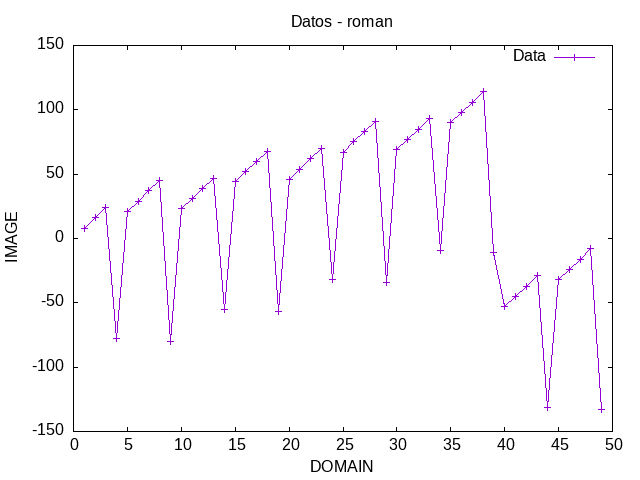
\includegraphics[width=0.3\linewidth]{img/roman/roman(49).png}}
    \subfloat[1 to 99]{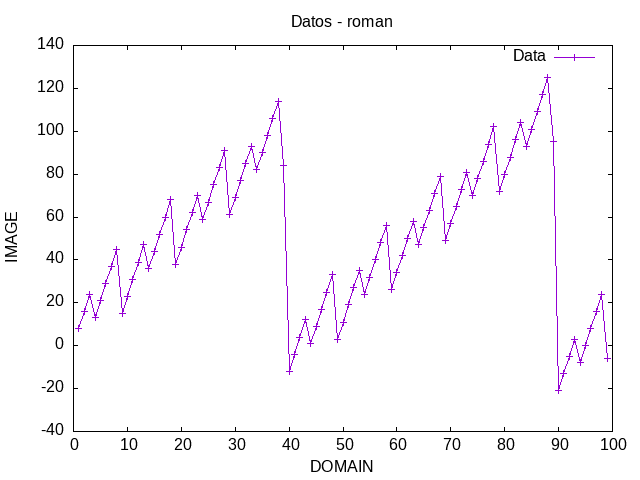
\includegraphics[width=0.3\linewidth]{img/roman/roman(99).png}}
    \subfloat[1 to 399]{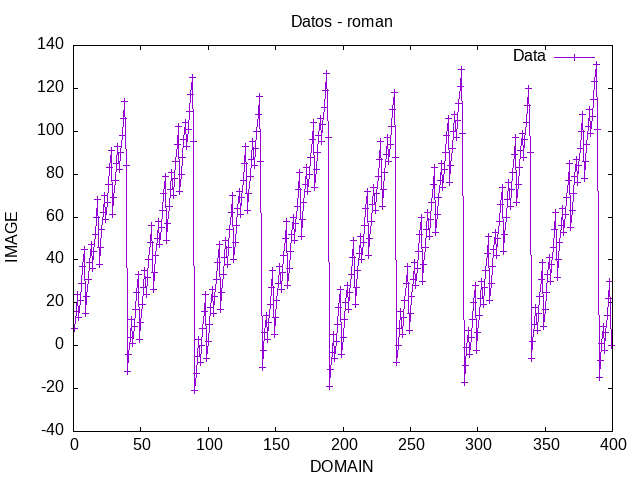
\includegraphics[width=0.3\linewidth]{img/roman/roman(399).png}}
    \caption{Distribution of the associated arabic number to the roman natural number}
    \label{romans}
\end{figure}\\
The function distribution that appears is the result of applying the function defined to the deterministic rules of roman numbers, therefore there is no knowledge of which is the function behind this process.\\
However is an ideal case to use the experimental observation and try to obtain with the dataset given by the deterministic method a function that approximates the distribution of the dataset.
\subsection{Analisis of the dataset and creation of the neural network} 
The shape of the function shown in \ref{romans} tend to mimic the \textit{Sawtooth wave} but, in this case, it is not exactly periodical.This consecuence (not been periodical) give some problems, because the application of the architecture develop to approximates the periodical functions can not be applied correctlly.\\
Despite this problem, it is possible to use the architeture develop for periodical functions (tending to approach the \textit{Fourier Serie} of the \textit{Sawthooth wave}) in what seems to be the period of the wave $49$. \\
Therefore, the neural neural network will have the architecture shown in \ref{roman-architecture}.
\begin{figure}[h]
    \begin{minipage}{5.5cm}
        \begin{center}
            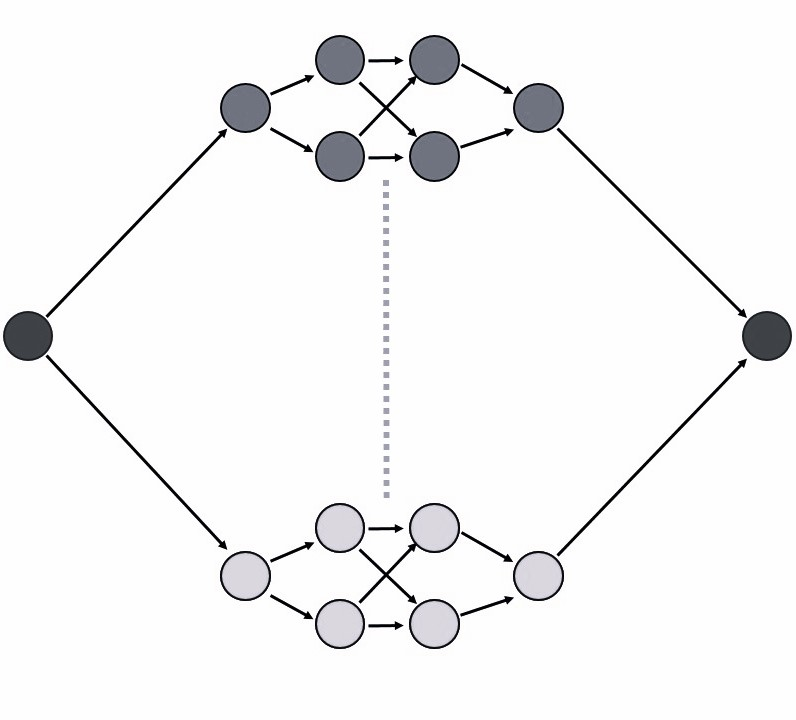
\includegraphics[width = 1\linewidth]{Neural_Network/roman_architecture.jpg}
            \caption{Proposal architecture of the neural network that approximates the roman number distribution}
            \label{roman-architecture}
        \end{center}
    \end{minipage}
    \hspace{1em}
    \begin{minipage}{9cm}
        This neural network will be composed by two neurons (one input and one output) that send/recive the information to/from sub-neural networks with the architecture obtained to modelate the $\sin$ function.\\
        The neural network will be trained with only the first subset of the dataset (number between 0 and 49) and if a bigger number is introduced it only needs to be reduced as the remainder of the division of this number and the period ($49$).\\
        The important part part of the network is the number of sub-neural networks, the learning rate and the number of epochs that needs to approximate properly the distribution.\\
        Unfortunately the number of epochs and learning rate can not be deduced until several have been tested.
    \end{minipage}
\end{figure}\\
However, the number of sub-networks could be deduced as the amount needes to approximate the \textit{Fourier Serie} the \textit{Sawthooth wave} with enough precission.\\
To test and deduce the optimal number of sub-networks and the value of the learnning rate, two first approached have been done, as can be seen in \ref{first-approach}
\begin{figure}[h]
    \centering
    \subfloat[Network with 3 architectures $1-2-2-1$ and fixed learning rate]{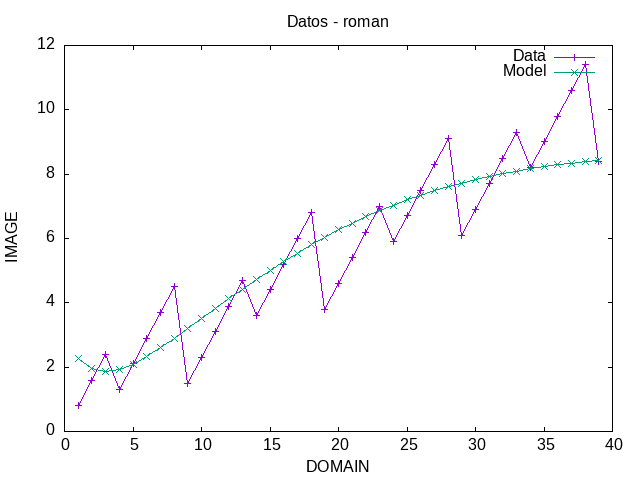
\includegraphics[width=0.45\linewidth]{img/roman/roman_first_approach.png}}
    \hspace{1em}
    \subfloat[Network with 4 architectures $1-2-2-1$ and decreassing learning rate]{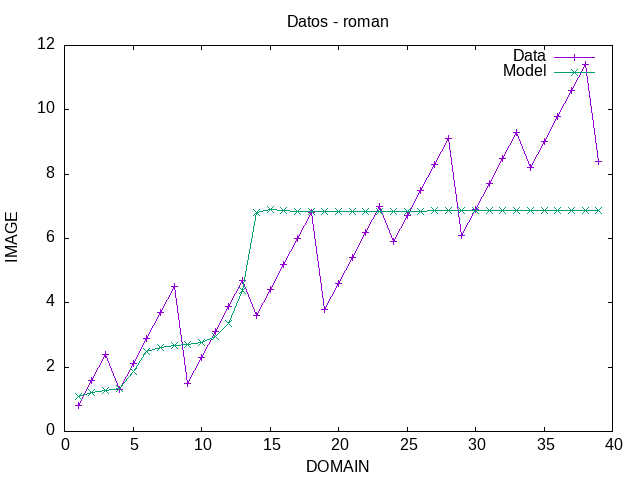
\includegraphics[width=0.45\linewidth]{img/roman/roman_second_approach.png}}
    \caption{Test of diferents neural networks to approach the distribution of roman numbers}
    \label{first-approach}
\end{figure}\\
The conclusion obtained from this tests is that the simple architecture of the $\sin$ function of $1-2-2-1$ is not enought and could be improven by using the most robust one of $1-2-4-1$.\\
Moreover, the variable learning rate (decreaseing it value while the epochs increases) adjust better the pics of the distribution. Although, the number of epochs testes (in case of figure \ref{first-approach} $1000$) seems to not being enought.\\
Also comment that the scale of the distribution has been decrease in one order of magnitude to reduce the ariance between values and help to focus the Backpropagation when training (by reducing the gradient vector and avoid irrational move thought the function cost reduction).
\begin{figure}[h]
    \begin{minipage}{5.5cm}
        \begin{center}
            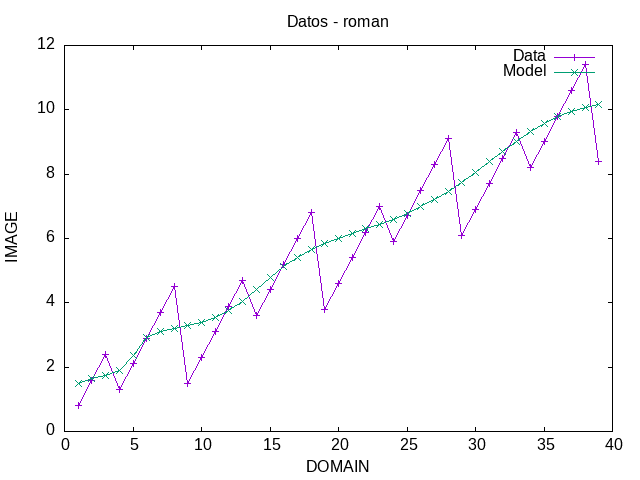
\includegraphics[width = 1 \linewidth]{img/roman/roman_third_approach.png}
            \caption{}
            \label{second-approach}
        \end{center}
    \end{minipage} \hspace{1em}
    \begin{minipage}{9cm}
        If the test is repeated with 4 sub-networks with architectures $1-2-4-1$, introducing the learning rate reduction by one order of magnitude each time the number of epochs done increases it order of magnitude and $10000$ epochs the results obtained perfoms a better approach, as can be seen in \ref{second-approach}.\\
        From the figure it is possible to deduce that the critical number of sub-networks has not been obtained yet. Moreover, observing the graph another conclusion can be made; the number of epochs is not enought.\\
        To obtain a usefull solution and (at least) an upper bound to the problem, and "overkill" architecure will be testes. 
    \end{minipage}
\end{figure}
\begin{figure}[h]
    \begin{minipage}{5.5cm}
        \begin{center}
            \includegraphics[width = 1 \linewidth]{img/roman/roman_third_approach.png}
            \caption{}
            \label{overkill-approach}
        \end{center}
    \end{minipage} \hspace{1em}
    \begin{minipage}{9cm}
        In this approach the number of epochs has been increased to $10^9$ epochs and includes $15$ sub-networks with architectures $1-2-4-1$.\\
        The results obtained in \ref{overkill-approach} are ......
    \end{minipage}
\end{figure}
\subsection{Efficiency and time-cost results}
To sum up all four tests done we can reflex its results in the table \ref{efficiency-table}.
\begin{table}[h]
    \centering
    \begin{tabular}{c|c|c|c|c|c}
        Sub-networks & Architecture & Epochs & Learning rate & Training time & Mean MSE\\\hline\hline
        3 & $1-2-2-1$ & $10^3$ & 0.01 & & 4.09 \\\hline
        4 & $1-2-2-1$ & $10^3$ & $\{10^{-2}, 10^{-3}\}$ & & 2.96 \\\hline
        4 & $1-2-4-1$ & $10^5$ & $\{10^{-(2+i)}\}_{i=0}^{2}$& & 0.87 \\\hline
        15 & $1-2-4-1$ & $10^9$ & $\{10^{-(3+2i)}\}_{i=0}^{3}$& & \\
    \end{tabular}
    \caption{}
    \label{efficiency-table}
\end{table}



\newpage
\begin{thebibliography}{X}
\bibitem{WIKIPEDIA-MLP} \textsc{Wikipedia},
\textit{Multilayer perceptron},\\ \url{https://en.wikipedia.org/wiki/Multilayer_perceptron}
\bibitem{WIKIPEDIA-PERCERPTRON} \textsc{Wikipedia},
\textit{Perceptrón},\\ \url{https://es.wikipedia.org/wiki/Perceptr%C3%B3n}
\bibitem{WIKIPEDIA-ACTIV.FUNCT,} \textsc{Wikipedia},
\textit{Activation function},\\ \url{https://en.wikipedia.org/wiki/Activation_function}
\bibitem{WIKIPEDIA-FRANK} \textsc{Wikipedia},
\textit{Frank Rosenblatt},\\ \url{https://es.wikipedia.org/wiki/Frank_Rosenblatt}
\bibitem{WIKIPEDIA-ACTIVATINGFUNCTION} \textsc{Wikipedia},
\textit{Activating Function},\\ \url{https://en.wikipedia.org/wiki/Activating_function}
\bibitem{WIKIPEDIA-ART.NN} \textsc{Wikipedia},
\textit{Artificial neural network},\\ \url{https://en.wikipedia.org/wiki/Artificial_neural_network}
\bibitem{WIKIPEDIA-NN} \textsc{Wikipedia},
\textit{Neural network},\\ \url{https://en.wikipedia.org/wiki/Neural_network}
\bibitem{WIKIPEDIA-SIGMOID_TEOREM} \textsc{Wikipedia},
\textit{Universal Approximation Theorem},\\ \url{https://en.wikipedia.org/wiki/Universal_approximation_theorem}
\bibitem{WIKIPEDIA-MSE} \textsc{Wikipedia},
\textit{Mean Squared Error},\\ \url{https://en.wikipedia.org/wiki/Mean_squared_error}
\bibitem{WIKIPEDIA-MAE} \textsc{Wikipedia},
\textit{Mean Absolute Error},\\ \url{https://en.wikipedia.org/wiki/Mean_absolute_error}
\bibitem{WIKIPEDIA-CE} \textsc{Wikipedia},
\textit{Cross-Entropy},\\ \url{https://en.wikipedia.org/wiki/Cross-entropy}
\bibitem{WIKIPEDIA-BACKPROP} \textsc{Wikipedia},
\textit{BackPropagation},\\ \url{https://en.wikipedia.org/wiki/Backpropagation}

\bibitem{Dan} \textsc{Dantzig, G.B.} y \textsc{P. Wolfe},
<<Decomposition principle for linear programs>>,
\textit{Operations Research}, \textbf{8}, págs. 101--111, 1960.

\end{thebibliography}
\end{document}
